\section{MOSFET Grundschaltungen}
Es werden drei Grundschaltungen unterschieden. 
Diese werden jeweils durch deren Common-Anschluss benannt.

\begin{center}
    \begingroup\rowcolors{1}{white}{gray!25}
    \begin{tabular}{|c|ccc|}
        \hline
        Schaltung   & Source-Schaltung & Gate-Schaltung & Drain-Schaltung \\
        \hline
        Common      & Source    & Gate      & Drain     \\
        Eingang     & Gate      & Source    & Gate      \\
        Ausgang     & Drain     & Drain     & Source    \\
        \hline
    \end{tabular}\endgroup
\end{center}

\textbf{Hinweis:} Die Drain-Schaltung wird auch Source-Follower genannt.


\subsection{Einsatzgebiete und Eigenschaften}

\begin{center}
    \begingroup\rowcolors{1}{white}{gray!25}
    \begin{tabular}{|c|ccc|}
        \hline
        Grundschaltung  & Anwendung                                 & $r_{\rm in}$  & $r_{\rm out}$ \\
        \hline
        Source          & Verstärker: Tiefe -- mittlere Frequenzen  & gross         & gross         \\
        Gate            & Verstärker: Hohe Freqenzen                & klein         & gross         \\
        Drain           & Spannungsfolger, Treiber, Impedanzwandler & gross         & klein         \\
        \hline
    \end{tabular}\endgroup
\end{center}

\subsection{Dimensionierung einer Gundschaltung -- Vorgehen}
\begin{easylist}
    \ListProperties(Style1*=\bfseries,Numbers2=l,Mark1={},Mark2={)},Indent2=1em)
    @ Arbeitspunkt mittels Grossignalersatzschaltung bestimmen (\ref{Grosssignalersatzschaltung} / \ref{Bestimmung des Arbeitspunkts})
    @ Kleinsignalersatzschaltung 
    @@ Beschaltung umzeichnen
    @@ Transistor durch Ersatzschaltbild ersetzen (\ref{Kleinsignalersatzschaltung})
    @ Durch lineare Analyse $a$ und $r$ berechnen
\end{easylist}

\subsection{Source-Schaltung}

Die Source-Schaltung ist eine \textbf{invertierende Verstärkerschaltung.}

\smallskip

\begin{minipage}[t]{0.4\columnwidth}
    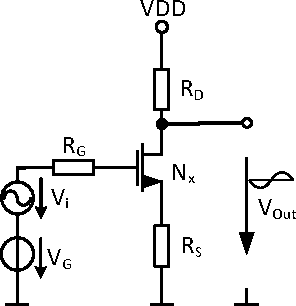
\includegraphics[width=\columnwidth, align=t]{images/03_source_schaltung.pdf}
\end{minipage}
\hfill
\begin{minipage}[t]{0.58\columnwidth}
    \subsubsection{Verstärkung}

    \vspace{-0.2cm}
    \[
        a = \frac{v_{\rm out}}{v_{\rm in}} = \frac{R_D}{R_S + \frac{1}{g_m} + \frac{g_0}{g_m}(R_D + R_S)} 
    \]


    \paragraph{Spezialfall}

    \vspace{-0.5cm}

    \[
        \boldsymbol{ R_S = 0 \qquad  a \approx - g_m \cdot R_{\rm out} \underbrace{= - g_m (r_{DS} \parallel R_D) }_{\text{Mikroelektronik}} }
    \]
    

    % $$g_m \gg g_0$ \& $R_D \ll r_{DS} \qquad a \approx - g_m \frac{R_D}{g_m R_D + 1} $$   % NOTE: Aus Skript (nicht in Vorlesung), macht Formatierung kaputt daher weggelassen, da allg. Formel immer gültig

    \vspace{-0.2cm}

    \paragraph{Optimierung}

    \begin{itemize}
        \item Maximierung der Verstärkung: \\
            $R_D \to \infty$ (so gross wie möglich) und $R_S \to 0$
        \item Chipplatz sparen: $R_S$ und $R_D$ weglassen
    \end{itemize}
\end{minipage}


\subsubsection{Designpraxis -- Strong Inversion}

Die \textbf{\myul{theoretisch}} maximal mögliche Verstärkung in strong inversion ergibt sich als

\vspace{-0.2cm}

\[
    a_{\rm max} = - \frac{g_m}{g_0} = -g_m r_{DS} = -\frac{2\cdot a_E \cdot L}{V_{GS} - V_T}
\]
% \[
%     r_{DS} = \frac{a_E \cdot L}{I_D} \qquad g_m = \mu C_{OX} \frac{W}{L} (V_{GS} - V_T) = \frac{2 I_D}{V_{GS}-V_T}
% \]


Damit der Wert $a_{\rm max}$ maximal wird, folgt as obiger Formel:

\smallskip

\begin{minipage}[t]{0.35\columnwidth}
    \begin{itemize}
        \item $g_m$ so gross wie möglich
        \item $r_{DS}$ so gross wie möglich
    \end{itemize}
\end{minipage}
\hfill
\begin{minipage}[t]{0.62\columnwidth}
    \begin{itemize}
        \item $V_{GS}$ so tief wie möglich  ($V_{GS}-V_T \approx 150 - \qty{200}{\milli\volt}$).
        \item $L$ möglichst gross \textrightarrow\ grosser Lastwiderstand
    \end{itemize}
\end{minipage}



\subsubsection{Designpraxis -- Weak Inversion}

Die \textbf{\myul{theoretisch}} maximal mögliche Verstärkung in weak inversion ergibt sich als

\vspace{-0.2cm}

\[
    a_{\rm max} = - \frac{g_m}{g_0} = -g_m r_{DS} = -\frac{a_E \cdot L}{n_m - V_{\rm temp}}
\]

% \[
%     g_{m} = \frac{I_D}{n_m V_{temp}} \qquad r_{DS} \approx \frac{a_E \cdot L}{I_D}
% \]

\begin{itemize}
    \item In weak inversion erreicht der Transistor seine maximale Verstärkung.
    \item Sie wird durch Technologieparameter sowie $L$ bestimmt.
    \item Da in weak inversion mit Nähreungsformeln gerechnet wird, muss simuliert werden.
\end{itemize}



\subsection{Gate-Schaltung}

Die Gate-Schaltung ist eine \textbf{nichtinvertierende Verstärkerschaltung.}

\smallskip

\begin{minipage}[t]{0.4\columnwidth}
    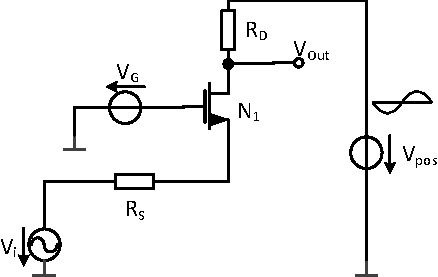
\includegraphics[width=\columnwidth, align=t]{images/03_gate_schaltung.pdf}
\end{minipage}
\hfill
\begin{minipage}[t]{0.58\columnwidth}
    \subsubsection{Verstärkung}

    \vspace{-0.2cm}

    \[
        a = \frac{v_{\rm out}}{v_{\rm in}} = \frac{R_D (1+\frac{g_0}{g_m})}{R_S + \frac{1}{g_m} + \frac{g_0}{g_m} (R_D + R_S)}
    \]

    \paragraph{Spezialfall}
    
    \vspace{-0.3cm}

    \[
        R_S = 0 \qquad  a \approx g_m \cdot R_{\rm out} \underbrace{= g_m (r_{DS} \parallel R_D) }_{\text{Mikroelektronik}} 
    \]
\end{minipage}

\smallskip

Für $R_S = 0$ und $R_D \ll r_{DS}$ gilt (ebenfalls in \textbf{strong inversion}) weiter: 
\[
    a \overset{R_D \text{klein}}{\approx} g_m R_D \qquad \text{bzw.} \qquad a \overset{R_D \text{gross}}{\approx} \frac{g_m}{g_0} \approx a_{\rm max}
\]

%TODO: [Flurin] Weak inversion Grenzwerte? Oder einfach Verweis auf Source-Schaltung?
% [Simi] @Flurin: Ich habe die folgende subsubsection etwas ergänzt. Ich danke, das sollte genügend Information sein

\subsubsection{Bemerkungen}
\begin{itemize}
    \item Bei den gegebenen Formeln wurde der \textbf{Body-Effekt vernachlässigt!}
    \item Ohne Body-Effekt erreicht die Gate-Schaltung die gleiche theoretisch maximal mögliche Verstärkung $a_{\rm max}$ wie die Source-Schaltung.
        Allerdings ist das Frequenzverhalten der Gate-Schaltung besser.
    \item Bei der Gate-Schaltung wird der Body-Effekt schnell zum Problem.
\end{itemize}



\subsection{Drain-Schaltung (Source-Follower)}

Die Drain-Schaltung ist eine \textbf{nichtinvertierende Verstärkerschaltung.}

\smallskip

\begin{minipage}[t]{0.4\columnwidth}
    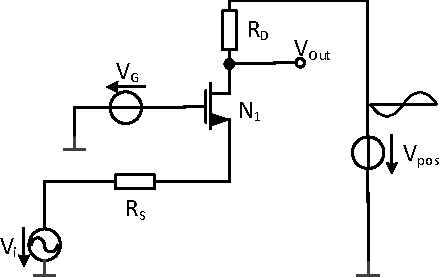
\includegraphics[width=\columnwidth, align=t]{images/03_drain_schaltung.pdf}
\end{minipage}
\hfill
\begin{minipage}[t]{0.58\columnwidth}
    \subsubsection{Verstärkung}

    \vspace{-0.2cm}
    \[
        a = \frac{v_{\rm out}}{v_{\rm in}} = \frac{R_S}{R_S + \frac{1}{g_m} + \frac{g_0}{g_m} (R_D + R_S)}
    \]

    \paragraph{Maximale Verstärkung}

    Für die \textbf{theoretisch} maximal mögliche Verstärkung $a_{\rm max}$ gilt für
    $g_m \ll g_0$ und $r_{DS} \ll R_D$

    \vspace{-0.2cm}

    \[
        a_{\rm max} = \lim_{R_S \to \infty} a = \lim_{R_S \to \infty} g_m \frac{R_S}{g_m R_S + 1} = 1
    \]
\end{minipage}


\subsubsection{Level-Shift}
Die Drain-Schaltung reduziert den DC-Pegel des Ausgangssignals um die Spannung $V_{GS}$. Somit ergibt sich der Zusammenhang:
\[
    V_{\rm in} - V_{\rm out} =  V_{GS} = V_T + \sqrt{\frac{2 I_D}{\mu C_{ox} \frac{W}{L}}} \qquad \Leftrightarrow\ \quad  V_{\rm out} = V_{\rm in} - \left( V_T + \sqrt{\frac{2 I_D}{\mu C_{ox} \frac{W}{L}}} \right)
\]
Damit der Level-Shift möglichst klein ist, wird $L$ möglichst gross gewählt.


\paragraph{Body Effekt}
Da die Source nicht auf Bulk-Potential ist, muss die Veränderung der Threshold Spannung $V_T$ aufgrund des Body-Effekts berücksichtigt werden (\ref{Strong Inversion}).


\subsubsection{Bemerkungen}
\begin{itemize}
    \item Der Source-Follower hat immer eine Verstärkung $a \leq 1$
    \item Der Source-Follower bewirkt immer einen Level-Shift um $V_{GS}$.
\end{itemize}



\subsection{Eingangs- und Ausgangswiderstände}

\subsubsection{Generelles Vorgehen}

\begin{itemize}
    \item Fiktive Spannungsquelle an entsprechenden Anschluss (z.B. Source) im Kleinsignalersatzschaltbild anschliessen.
    \item Strom, der über den Anschluss (z.B. Source) in den in den Transistor fliesst, messen.
    \item Widerstand als $r_i = \abs{ \frac{u_i}{i_i} }$ berechnen.
\end{itemize}


\subsubsection{Eingangs- und Ausgangswiderstände berechnen}

\paragraph{Gate $\bm{r_{i,G}}$}

\vspace{-0.2cm}

\[
    r_{i, G} \to\ \infty
\]


\paragraph{Source $\bm{r_{i,S}}$}

\vspace{-0.3cm}

\begin{align*}
    \text{Allgemein}            & \qquad r_{i, S} = \left( \frac{1}{g_m} \parallel r_{DS} \right) \left( 1 + \frac{R_D}{r_{DS}} \right) = \frac{1}{g_m + g_0} (1 + g_0 R_D) \\
    \text{Für } r_{DS} \gg R_D  & \qquad r_{i, S} \approx \frac{1}{g_m} \parallel r_{DS} = \frac{1}{g_m + g_0} \\
    \text{Für } g_m \gg g_0     & \qquad r_{i, S} \approx \frac{1}{g_m}
\end{align*}


\paragraph{Drain $\bm{r_{i,D}}$}

\vspace{-0.3cm}

\begin{align*}
    \text{Allgemein}            & \qquad r_{i, D} = r_{DS} \left( 1 + g_m R_S + \frac{R_S}{r_{DS}} \right) = \frac{1}{g_0} (1+g_m R_S) + R_S \\
    \text{Für } r_{DS} \gg R_S  & \qquad r_{i, D} \approx r_{DS} \left( 1 + g_m R_S \right) = \frac{1}{g_0} (1+g_m R_S) + R_S \\
    \text{Für } R_S = 0         & \qquad r_{i, D} \approx r_{DS} = \frac{1}{g_0}
\end{align*}

\columnbreak

